\chapter{Database Diagrams}
\label{chapter:diagrams}

\section{Models and relationships}
The diagrams should be simple enough to be self-explanatory. The DMD is created first and based on the many-to-many relationship between hotels and facilities, it gives rise to an index table (HotelFacilities).
In the DMD, HotelFacilities is not considered as an independent entity but rather as a way to manage the relationship between Hotel and Facilities.
The ERD is then created from the DMD and shows the relationships between the tables, their PK, FK, and data types.

\subsection{Domain Model Diagram}
See figure \ref*{fig:domain-model-diagram}. 
This DMD only contains entities, multiplicities, and relationships.
This provides input on how the database should be designed based on the individual tables and their relationships to each other.

\begin{figure}
  \centering
  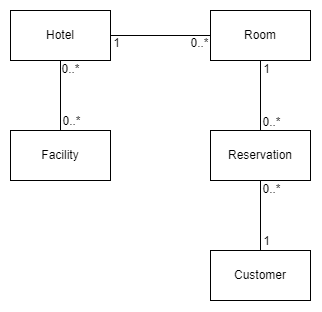
\includegraphics[width=0.75\textwidth]{figures/SWD_Domain_HotelManagement.png}
  \caption{Domain Model Diagram}
  \label{fig:domain-model-diagram}
\end{figure}

\pagebreak

\subsection{Entity-Relationship Diagram}
See figure \ref*{fig:entity-relationship-diagram}. 
The ERD is generated from the tables in the database and shows the relationships between the tables, their PK, FK, and data types.

\begin{figure}
  \centering
  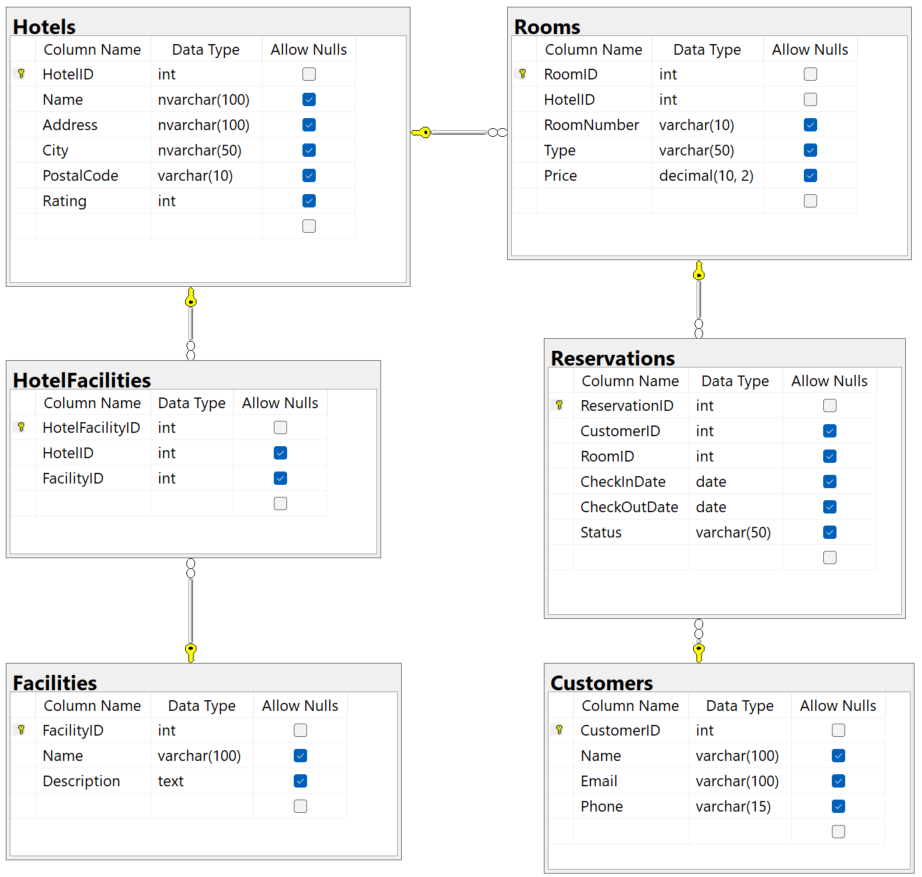
\includegraphics[width=0.75\textwidth]{figures/SWD_ERD_HotelManagement.png}
  \caption{Entity Relationship Diagram}
  \label{fig:entity-relationship-diagram}
\end{figure}